\documentclass[border={6pt 6pt 6pt 6pt}]{standalone}
\usepackage[default]{lato}
\usepackage{tikz,xcolor,times}
\usetikzlibrary{shapes,arrows,calc,shadows.blur,arrows.meta}
\definecolor{uogblue}{HTML}{003865}
\definecolor{uogsky}{HTML}{005398}
\definecolor{uogcobalt}{HTML}{0075B0}
\definecolor{uogturquoise}{HTML}{00B5D1}
\definecolor{uogslate}{HTML}{4F5961}
\definecolor{uogleaf}{HTML}{00843D}
\definecolor{uogmoss}{HTML}{385A4F}
\definecolor{uogsandstone}{HTML}{7A6855}
\definecolor{uogmocha}{HTML}{AA8066}
\definecolor{uogburgundy}{HTML}{7D2239}
\definecolor{uogpillarbox}{HTML}{B30C00}
\definecolor{uoglavender}{HTML}{5B4D94}
\definecolor{uogthistle}{HTML}{951272}
\definecolor{uogrose}{HTML}{B06C96}
\definecolor{uogrust}{HTML}{BE4D00}
\definecolor{uogpumpkin}{HTML}{FFB948}
\definecolor{uogsunshine}{HTML}{FFDC36}
\begin{document}
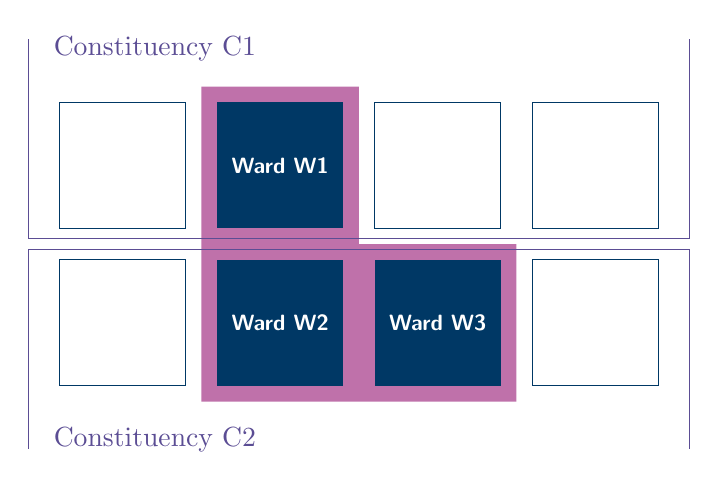
\begin{tikzpicture}[scale=0.4]
\fill[fill=uogthistle!60] (-0.5,-0.5) -- (-0.5, 9.5) -- (4.5,9.5) -- (4.5,4.5) -- (9.5, 4.5) -- (9.5,-0.5) -- cycle;
\draw[uogblue] (-5,0) rectangle (-1,4);
\draw[uogblue] (-5,5) rectangle (-1,9);
\draw[uogblue] (5,5) rectangle (9,9);
\draw[uogblue] (10,0) rectangle (14,4);
\draw[uogblue] (10,5) rectangle (14,9);
\fill[uogblue] (0,5) rectangle (4,9); \node[white] at (2,7) {\sffamily \bfseries \footnotesize Ward W1};
\fill[uogblue] (0,0) rectangle (4,4); \node[white] at (2,2) {\sffamily \bfseries \footnotesize Ward W2};
\fill[uogblue]  (5,0) rectangle (9,4); \node[white] at (7,2) {\sffamily \bfseries \footnotesize Ward W3};
\draw[uoglavender] (-6,11) -- (-6,4.67) -- (15,4.67) -- (15,11);
\draw[uoglavender] (-6,-2) -- (-6,4.33) -- (15,4.33) -- (15,-2);
\node[align=left,anchor=south west,uoglavender] at (-5.5,10) {Constituency C1};
\node[align=left,anchor=north west,uoglavender] at (-5.5,-1) {Constituency C2};
\end{tikzpicture}
\end{document}
